% Supplementary Figure S1 - scaling benchmarks.
% Source of truth for the caption: ../benchmarks/SUPPLEMENTARY_TEXT.md
% Graphic: ../benchmarks/figS_scaling.pdf (vector, no raster, fonts embedded,
% 242.5 x 80.6 mm -> 56.5 mm of height at BMC's 170 mm full width).
% Requires: graphicx
% Numbering: see the note in figure_s2.tex about \thefigure for the supplement.
\begin{figure}[t!]
\centering
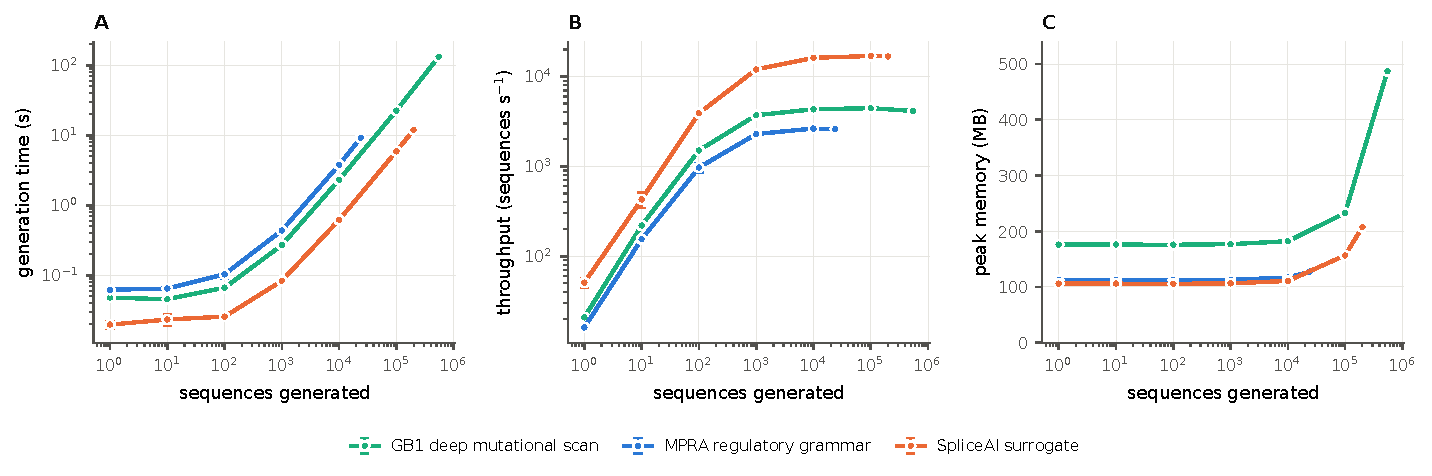
\includegraphics[width=\textwidth]{../benchmarks/figS_scaling}
\caption{\textbf{Library generation scales linearly in time and memory.}
\textbf{(A)} Wall-clock generation time, \textbf{(B)} throughput, and
\textbf{(C)} peak resident memory against the number of sequences generated, for
the three worked examples. Points are means of 5 replicate runs; error bars show
$\pm$1~SD and are smaller than the plotting symbols at most points. Below
$\sim$10$^3$ sequences a fixed setup cost dominates, giving the plateau in
\textbf{(A)} and the rise in \textbf{(B)}; above 10$^4$ sequences throughput is
constant, so generation time is linear in library size. Peak memory increases
linearly, by 0.52--0.66~kB per sequence above a $\sim$106~MB baseline.}
\label{fig:figureS1}
\end{figure}
